% GNUPLOT: LaTeX picture with Postscript
\begingroup
  \makeatletter
  \providecommand\color[2][]{%
    \GenericError{(gnuplot) \space\space\space\@spaces}{%
      Package color not loaded in conjunction with
      terminal option `colourtext'%
    }{See the gnuplot documentation for explanation.%
    }{Either use 'blacktext' in gnuplot or load the package
      color.sty in LaTeX.}%
    \renewcommand\color[2][]{}%
  }%
  \providecommand\includegraphics[2][]{%
    \GenericError{(gnuplot) \space\space\space\@spaces}{%
      Package graphicx or graphics not loaded%
    }{See the gnuplot documentation for explanation.%
    }{The gnuplot epslatex terminal needs graphicx.sty or graphics.sty.}%
    \renewcommand\includegraphics[2][]{}%
  }%
  \providecommand\rotatebox[2]{#2}%
  \@ifundefined{ifGPcolor}{%
    \newif\ifGPcolor
    \GPcolortrue
  }{}%
  \@ifundefined{ifGPblacktext}{%
    \newif\ifGPblacktext
    \GPblacktexttrue
  }{}%
  % define a \g@addto@macro without @ in the name:
  \let\gplgaddtomacro\g@addto@macro
  % define empty templates for all commands taking text:
  \gdef\gplbacktext{}%
  \gdef\gplfronttext{}%
  \makeatother
  \ifGPblacktext
    % no textcolor at all
    \def\colorrgb#1{}%
    \def\colorgray#1{}%
  \else
    % gray or color?
    \ifGPcolor
      \def\colorrgb#1{\color[rgb]{#1}}%
      \def\colorgray#1{\color[gray]{#1}}%
      \expandafter\def\csname LTw\endcsname{\color{white}}%
      \expandafter\def\csname LTb\endcsname{\color{black}}%
      \expandafter\def\csname LTa\endcsname{\color{black}}%
      \expandafter\def\csname LT0\endcsname{\color[rgb]{1,0,0}}%
      \expandafter\def\csname LT1\endcsname{\color[rgb]{0,1,0}}%
      \expandafter\def\csname LT2\endcsname{\color[rgb]{0,0,1}}%
      \expandafter\def\csname LT3\endcsname{\color[rgb]{1,0,1}}%
      \expandafter\def\csname LT4\endcsname{\color[rgb]{0,1,1}}%
      \expandafter\def\csname LT5\endcsname{\color[rgb]{1,1,0}}%
      \expandafter\def\csname LT6\endcsname{\color[rgb]{0,0,0}}%
      \expandafter\def\csname LT7\endcsname{\color[rgb]{1,0.3,0}}%
      \expandafter\def\csname LT8\endcsname{\color[rgb]{0.5,0.5,0.5}}%
    \else
      % gray
      \def\colorrgb#1{\color{black}}%
      \def\colorgray#1{\color[gray]{#1}}%
      \expandafter\def\csname LTw\endcsname{\color{white}}%
      \expandafter\def\csname LTb\endcsname{\color{black}}%
      \expandafter\def\csname LTa\endcsname{\color{black}}%
      \expandafter\def\csname LT0\endcsname{\color{black}}%
      \expandafter\def\csname LT1\endcsname{\color{black}}%
      \expandafter\def\csname LT2\endcsname{\color{black}}%
      \expandafter\def\csname LT3\endcsname{\color{black}}%
      \expandafter\def\csname LT4\endcsname{\color{black}}%
      \expandafter\def\csname LT5\endcsname{\color{black}}%
      \expandafter\def\csname LT6\endcsname{\color{black}}%
      \expandafter\def\csname LT7\endcsname{\color{black}}%
      \expandafter\def\csname LT8\endcsname{\color{black}}%
    \fi
  \fi
    \setlength{\unitlength}{0.0500bp}%
    \ifx\gptboxheight\undefined%
      \newlength{\gptboxheight}%
      \newlength{\gptboxwidth}%
      \newsavebox{\gptboxtext}%
    \fi%
    \setlength{\fboxrule}{0.5pt}%
    \setlength{\fboxsep}{1pt}%
    \definecolor{tbcol}{rgb}{1,1,1}%
\begin{picture}(6980.00,6980.00)%
    \gplgaddtomacro\gplbacktext{%
    }%
    \gplgaddtomacro\gplfronttext{%
      \csname LTb\endcsname%%
      \put(389,3994){\makebox(0,0)[r]{\strut{}$-160$}}%
      \csname LTb\endcsname%%
      \put(389,4326){\makebox(0,0)[r]{\strut{}$-120$}}%
      \csname LTb\endcsname%%
      \put(389,4659){\makebox(0,0)[r]{\strut{}$-80$}}%
      \csname LTb\endcsname%%
      \put(389,4991){\makebox(0,0)[r]{\strut{}$-40$}}%
      \csname LTb\endcsname%%
      \put(389,5324){\makebox(0,0)[r]{\strut{}$0$}}%
      \csname LTb\endcsname%%
      \put(389,5656){\makebox(0,0)[r]{\strut{}$40$}}%
      \csname LTb\endcsname%%
      \put(389,5989){\makebox(0,0)[r]{\strut{}$80$}}%
      \csname LTb\endcsname%%
      \put(389,6321){\makebox(0,0)[r]{\strut{}$120$}}%
      \csname LTb\endcsname%%
      \put(389,6654){\makebox(0,0)[r]{\strut{}$160$}}%
      \csname LTb\endcsname%%
      \put(487,3652){\makebox(0,0){\strut{}}}%
      \csname LTb\endcsname%%
      \put(986,3652){\makebox(0,0){\strut{}}}%
      \csname LTb\endcsname%%
      \put(1484,3652){\makebox(0,0){\strut{}}}%
      \csname LTb\endcsname%%
      \put(1983,3652){\makebox(0,0){\strut{}}}%
      \csname LTb\endcsname%%
      \put(2482,3652){\makebox(0,0){\strut{}}}%
      \csname LTb\endcsname%%
      \put(2981,3652){\makebox(0,0){\strut{}}}%
      \csname LTb\endcsname%%
      \put(3480,3652){\makebox(0,0){\strut{}}}%
      \csname LTb\endcsname%%
      \put(32,5324){\rotatebox{-270.00}{\makebox(0,0){\normalsize $\Psi$}}}%
      \csname LTb\endcsname%%
      \put(1669,5498){\rotatebox{-63.00}{\makebox(0,0){\strut{}\textcolor{black}{\footnotesize 500}}}}%
      \csname LTb\endcsname%%
      \put(2272,5409){\rotatebox{130.00}{\makebox(0,0){\strut{}\textcolor{black}{\footnotesize 400}}}}%
      \csname LTb\endcsname%%
      \put(1758,5160){\rotatebox{-46.00}{\makebox(0,0){\strut{}\textcolor{black}{\footnotesize 400}}}}%
      \csname LTb\endcsname%%
      \put(1725,5940){\rotatebox{157.00}{\makebox(0,0){\strut{}\textcolor{black}{\footnotesize 300}}}}%
      \csname LTb\endcsname%%
      \put(1870,4897){\rotatebox{-39.00}{\makebox(0,0){\strut{}\textcolor{black}{\footnotesize 300}}}}%
      \csname LTb\endcsname%%
      \put(2641,5261){\rotatebox{115.00}{\makebox(0,0){\strut{}\textcolor{black}{\footnotesize 200}}}}%
      \csname LTb\endcsname%%
      \put(1191,6171){\rotatebox{-140.00}{\makebox(0,0){\strut{}\textcolor{black}{\footnotesize 200}}}}%
      \csname LTb\endcsname%%
      \put(1989,4683){\rotatebox{-24.00}{\makebox(0,0){\strut{}\textcolor{black}{\footnotesize 200}}}}%
      \csname LTb\endcsname%%
      \put(1191,4995){\rotatebox{39.00}{\makebox(0,0){\strut{}\textcolor{black}{\footnotesize 100}}}}%
      \csname LTb\endcsname%%
      \put(1142,6544){\rotatebox{44.00}{\makebox(0,0){\strut{}\textcolor{black}{\footnotesize 100}}}}%
      \csname LTb\endcsname%%
      \put(2474,6418){\rotatebox{62.00}{\makebox(0,0){\strut{}\textcolor{black}{\footnotesize 100}}}}%
      \csname LTb\endcsname%%
      \put(2748,5336){\rotatebox{-73.00}{\makebox(0,0){\strut{}\textcolor{black}{\footnotesize 100}}}}%
      \csname LTb\endcsname%%
      \put(990,4433){\rotatebox{-33.00}{\makebox(0,0){\strut{}\textcolor{black}{\footnotesize 100}}}}%
      \csname LTb\endcsname%%
      \put(2588,4180){\rotatebox{-44.00}{\makebox(0,0){\strut{}\textcolor{black}{\footnotesize 100}}}}%
      \csname LTb\endcsname%%
      \put(585,5638){\rotatebox{-104.00}{\makebox(0,0){\strut{}\textcolor{black}{\footnotesize 50}}}}%
      \csname LTb\endcsname%%
      \put(1865,6569){\rotatebox{158.00}{\makebox(0,0){\strut{}\textcolor{black}{\footnotesize 50}}}}%
      \csname LTb\endcsname%%
      \put(1541,3978){\rotatebox{-72.00}{\makebox(0,0){\strut{}\textcolor{black}{\footnotesize 50}}}}%
      \csname LTb\endcsname%%
      \put(2926,5567){\rotatebox{-139.00}{\makebox(0,0){\strut{}\textcolor{black}{\footnotesize 50}}}}%
      \csname LTb\endcsname%%
      \put(1983,6943){\makebox(0,0){\strut{}Conformational Energy (meV)}}%
    }%
    \gplgaddtomacro\gplbacktext{%
    }%
    \gplgaddtomacro\gplfronttext{%
      \csname LTb\endcsname%%
      \put(3695,3994){\makebox(0,0)[r]{\strut{}}}%
      \csname LTb\endcsname%%
      \put(3695,4326){\makebox(0,0)[r]{\strut{}}}%
      \csname LTb\endcsname%%
      \put(3695,4659){\makebox(0,0)[r]{\strut{}}}%
      \csname LTb\endcsname%%
      \put(3695,4991){\makebox(0,0)[r]{\strut{}}}%
      \csname LTb\endcsname%%
      \put(3695,5324){\makebox(0,0)[r]{\strut{}}}%
      \csname LTb\endcsname%%
      \put(3695,5656){\makebox(0,0)[r]{\strut{}}}%
      \csname LTb\endcsname%%
      \put(3695,5989){\makebox(0,0)[r]{\strut{}}}%
      \csname LTb\endcsname%%
      \put(3695,6321){\makebox(0,0)[r]{\strut{}}}%
      \csname LTb\endcsname%%
      \put(3695,6654){\makebox(0,0)[r]{\strut{}}}%
      \csname LTb\endcsname%%
      \put(3793,3652){\makebox(0,0){\strut{}}}%
      \csname LTb\endcsname%%
      \put(4291,3652){\makebox(0,0){\strut{}}}%
      \csname LTb\endcsname%%
      \put(4790,3652){\makebox(0,0){\strut{}}}%
      \csname LTb\endcsname%%
      \put(5289,3652){\makebox(0,0){\strut{}}}%
      \csname LTb\endcsname%%
      \put(5788,3652){\makebox(0,0){\strut{}}}%
      \csname LTb\endcsname%%
      \put(6287,3652){\makebox(0,0){\strut{}}}%
      \csname LTb\endcsname%%
      \put(6785,3652){\makebox(0,0){\strut{}}}%
      \csname LTb\endcsname%%
      \put(5700,4218){\rotatebox{43.00}{\makebox(0,0){\strut{}\textcolor{black}{\footnotesize 3.0}}}}%
      \csname LTb\endcsname%%
      \put(5522,5222){\rotatebox{129.00}{\makebox(0,0){\strut{}\textcolor{black}{\footnotesize 2.5}}}}%
      \csname LTb\endcsname%%
      \put(4353,6459){\rotatebox{-72.00}{\makebox(0,0){\strut{}\textcolor{black}{\footnotesize 2.5}}}}%
      \csname LTb\endcsname%%
      \put(5372,6661){\makebox(0,0){\strut{}\textcolor{black}{\footnotesize 2.5}}}%
      \csname LTb\endcsname%%
      \put(4515,3989){\rotatebox{40.00}{\makebox(0,0){\strut{}\textcolor{black}{\footnotesize 2.5}}}}%
      \csname LTb\endcsname%%
      \put(5552,4386){\rotatebox{42.00}{\makebox(0,0){\strut{}\textcolor{black}{\footnotesize 2.5}}}}%
      \csname LTb\endcsname%%
      \put(6545,4794){\rotatebox{-22.00}{\makebox(0,0){\strut{}\textcolor{black}{\footnotesize 2.5}}}}%
      \csname LTb\endcsname%%
      \put(4187,6670){\rotatebox{-108.00}{\makebox(0,0){\strut{}\textcolor{black}{\footnotesize 2.0}}}}%
      \csname LTb\endcsname%%
      \put(4560,6009){\rotatebox{-4.00}{\makebox(0,0){\strut{}\textcolor{black}{\footnotesize 2.0}}}}%
      \csname LTb\endcsname%%
      \put(5567,6455){\rotatebox{-5.00}{\makebox(0,0){\strut{}\textcolor{black}{\footnotesize 2.0}}}}%
      \csname LTb\endcsname%%
      \put(5101,4265){\rotatebox{24.00}{\makebox(0,0){\strut{}\textcolor{black}{\footnotesize 2.0}}}}%
      \csname LTb\endcsname%%
      \put(5251,5011){\rotatebox{145.00}{\makebox(0,0){\strut{}\textcolor{black}{\footnotesize 2.0}}}}%
      \csname LTb\endcsname%%
      \put(5086,5696){\rotatebox{-23.00}{\makebox(0,0){\strut{}\textcolor{black}{\footnotesize 2.0}}}}%
      \csname LTb\endcsname%%
      \put(5973,5109){\rotatebox{-19.00}{\makebox(0,0){\strut{}\textcolor{black}{\footnotesize 2.0}}}}%
      \csname LTb\endcsname%%
      \put(4006,5346){\rotatebox{50.00}{\makebox(0,0){\strut{}\textcolor{black}{\footnotesize 1.5}}}}%
      \csname LTb\endcsname%%
      \put(4845,5166){\rotatebox{-50.00}{\makebox(0,0){\strut{}\textcolor{black}{\footnotesize 1.5}}}}%
      \csname LTb\endcsname%%
      \put(4906,4402){\rotatebox{-173.00}{\makebox(0,0){\strut{}\textcolor{black}{\footnotesize 1.5}}}}%
      \csname LTb\endcsname%%
      \put(6065,6324){\rotatebox{-155.00}{\makebox(0,0){\strut{}\textcolor{black}{\footnotesize 1.5}}}}%
      \csname LTb\endcsname%%
      \put(5236,5857){\rotatebox{-36.00}{\makebox(0,0){\strut{}\textcolor{black}{\footnotesize 1.5}}}}%
      \csname LTb\endcsname%%
      \put(6199,5401){\rotatebox{16.00}{\makebox(0,0){\strut{}\textcolor{black}{\footnotesize 1.5}}}}%
      \csname LTb\endcsname%%
      \put(3907,4143){\rotatebox{75.00}{\makebox(0,0){\strut{}\textcolor{black}{\footnotesize 1.0}}}}%
      \csname LTb\endcsname%%
      \put(4274,5214){\rotatebox{14.00}{\makebox(0,0){\strut{}\textcolor{black}{\footnotesize 1.0}}}}%
      \csname LTb\endcsname%%
      \put(4620,4529){\rotatebox{-156.00}{\makebox(0,0){\strut{}\textcolor{black}{\footnotesize 1.0}}}}%
      \csname LTb\endcsname%%
      \put(6003,6130){\rotatebox{-158.00}{\makebox(0,0){\strut{}\textcolor{black}{\footnotesize 1.0}}}}%
      \csname LTb\endcsname%%
      \put(6214,5602){\rotatebox{11.00}{\makebox(0,0){\strut{}\textcolor{black}{\footnotesize 1.0}}}}%
      \csname LTb\endcsname%%
      \put(4533,4880){\rotatebox{116.00}{\makebox(0,0){\strut{}\textcolor{black}{\footnotesize 0.5}}}}%
      \csname LTb\endcsname%%
      \put(5289,6943){\makebox(0,0){Dipole Strength (Debye)}}%
    }%
    \gplgaddtomacro\gplbacktext{%
    }%
    \gplgaddtomacro\gplfronttext{%
      \csname LTb\endcsname%%
      \put(389,723){\makebox(0,0)[r]{\strut{}$-160$}}%
      \csname LTb\endcsname%%
      \put(389,1055){\makebox(0,0)[r]{\strut{}$-120$}}%
      \csname LTb\endcsname%%
      \put(389,1388){\makebox(0,0)[r]{\strut{}$-80$}}%
      \csname LTb\endcsname%%
      \put(389,1720){\makebox(0,0)[r]{\strut{}$-40$}}%
      \csname LTb\endcsname%%
      \put(389,2053){\makebox(0,0)[r]{\strut{}$0$}}%
      \csname LTb\endcsname%%
      \put(389,2385){\makebox(0,0)[r]{\strut{}$40$}}%
      \csname LTb\endcsname%%
      \put(389,2718){\makebox(0,0)[r]{\strut{}$80$}}%
      \csname LTb\endcsname%%
      \put(389,3050){\makebox(0,0)[r]{\strut{}$120$}}%
      \csname LTb\endcsname%%
      \put(389,3383){\makebox(0,0)[r]{\strut{}$160$}}%
      \csname LTb\endcsname%%
      \put(487,380){\makebox(0,0){\strut{}$-180$}}%
      \csname LTb\endcsname%%
      \put(986,380){\makebox(0,0){\strut{}$-120$}}%
      \csname LTb\endcsname%%
      \put(1484,380){\makebox(0,0){\strut{}$-60$}}%
      \csname LTb\endcsname%%
      \put(1983,380){\makebox(0,0){\strut{}$0$}}%
      \csname LTb\endcsname%%
      \put(2482,380){\makebox(0,0){\strut{}$60$}}%
      \csname LTb\endcsname%%
      \put(2981,380){\makebox(0,0){\strut{}$120$}}%
      \csname LTb\endcsname%%
      \put(3479,380){\makebox(0,0){\strut{}$180$}}%
      \csname LTb\endcsname%%
      \put(32,2053){\rotatebox{-270.00}{\makebox(0,0){\normalsize $\Psi$}}}%
      \csname LTb\endcsname%%
      \put(1983,117){\makebox(0,0){\normalsize $\Phi$}}%
      \csname LTb\endcsname%%
      \put(1881,2279){\rotatebox{148.00}{\makebox(0,0){\strut{}\textcolor{black}{\footnotesize 1.3}}}}%
      \csname LTb\endcsname%%
      \put(1696,1928){\rotatebox{-45.00}{\makebox(0,0){\strut{}\textcolor{black}{\footnotesize 1.4}}}}%
      \csname LTb\endcsname%%
      \put(2297,2279){\rotatebox{143.00}{\makebox(0,0){\strut{}\textcolor{black}{\footnotesize 1.5}}}}%
      \csname LTb\endcsname%%
      \put(1947,1554){\rotatebox{-45.00}{\makebox(0,0){\strut{}\textcolor{black}{\footnotesize 1.5}}}}%
      \csname LTb\endcsname%%
      \put(1582,2824){\rotatebox{45.00}{\makebox(0,0){\strut{}\textcolor{black}{\footnotesize 1.6}}}}%
      \csname LTb\endcsname%%
      \put(2693,1629){\rotatebox{48.00}{\makebox(0,0){\strut{}\textcolor{black}{\footnotesize 1.6}}}}%
      \csname LTb\endcsname%%
      \put(883,2824){\rotatebox{-34.00}{\makebox(0,0){\strut{}\textcolor{black}{\footnotesize 1.7}}}}%
      \csname LTb\endcsname%%
      \put(1411,1040){\rotatebox{112.00}{\makebox(0,0){\strut{}\textcolor{black}{\footnotesize 1.7}}}}%
      \csname LTb\endcsname%%
      \put(2845,3372){\rotatebox{-135.00}{\makebox(0,0){\strut{}\textcolor{black}{\footnotesize 1.7}}}}%
      \csname LTb\endcsname%%
      \put(2754,783){\rotatebox{-25.00}{\makebox(0,0){\strut{}\textcolor{black}{\footnotesize 1.7}}}}%
      \csname LTb\endcsname%%
      \put(1983,3672){\makebox(0,0){VBA EA (eV)}}%
    }%
    \gplgaddtomacro\gplbacktext{%
    }%
    \gplgaddtomacro\gplfronttext{%
      \csname LTb\endcsname%%
      \put(3695,723){\makebox(0,0)[r]{\strut{}}}%
      \csname LTb\endcsname%%
      \put(3695,1055){\makebox(0,0)[r]{\strut{}}}%
      \csname LTb\endcsname%%
      \put(3695,1388){\makebox(0,0)[r]{\strut{}}}%
      \csname LTb\endcsname%%
      \put(3695,1720){\makebox(0,0)[r]{\strut{}}}%
      \csname LTb\endcsname%%
      \put(3695,2053){\makebox(0,0)[r]{\strut{}}}%
      \csname LTb\endcsname%%
      \put(3695,2385){\makebox(0,0)[r]{\strut{}}}%
      \csname LTb\endcsname%%
      \put(3695,2718){\makebox(0,0)[r]{\strut{}}}%
      \csname LTb\endcsname%%
      \put(3695,3050){\makebox(0,0)[r]{\strut{}}}%
      \csname LTb\endcsname%%
      \put(3695,3383){\makebox(0,0)[r]{\strut{}}}%
      \csname LTb\endcsname%%
      \put(3793,380){\makebox(0,0){\strut{}$-180$}}%
      \csname LTb\endcsname%%
      \put(4291,380){\makebox(0,0){\strut{}$-120$}}%
      \csname LTb\endcsname%%
      \put(4790,380){\makebox(0,0){\strut{}$-60$}}%
      \csname LTb\endcsname%%
      \put(5289,380){\makebox(0,0){\strut{}$0$}}%
      \csname LTb\endcsname%%
      \put(5788,380){\makebox(0,0){\strut{}$60$}}%
      \csname LTb\endcsname%%
      \put(6287,380){\makebox(0,0){\strut{}$120$}}%
      \csname LTb\endcsname%%
      \put(6785,380){\makebox(0,0){\strut{}$180$}}%
      \csname LTb\endcsname%%
      \put(5289,117){\makebox(0,0){\normalsize $\Phi$}}%
      \csname LTb\endcsname%%
      \put(5528,1735){\rotatebox{-34.00}{\makebox(0,0){\strut{}\textcolor{black}{\footnotesize 9}}}}%
      \csname LTb\endcsname%%
      \put(5878,726){\rotatebox{-22.00}{\makebox(0,0){\strut{}\textcolor{black}{\footnotesize 9}}}}%
      \csname LTb\endcsname%%
      \put(5637,1104){\rotatebox{69.00}{\makebox(0,0){\strut{}\textcolor{black}{\footnotesize 6}}}}%
      \csname LTb\endcsname%%
      \put(5502,2068){\rotatebox{-38.00}{\makebox(0,0){\strut{}\textcolor{black}{\footnotesize 6}}}}%
      \csname LTb\endcsname%%
      \put(6181,648){\rotatebox{-151.00}{\makebox(0,0){\strut{}\textcolor{black}{\footnotesize 6}}}}%
      \csname LTb\endcsname%%
      \put(4831,3035){\rotatebox{39.00}{\makebox(0,0){\strut{}\textcolor{black}{\footnotesize 3}}}}%
      \csname LTb\endcsname%%
      \put(5576,1294){\rotatebox{70.00}{\makebox(0,0){\strut{}\textcolor{black}{\footnotesize 3}}}}%
      \csname LTb\endcsname%%
      \put(5516,2146){\rotatebox{-39.00}{\makebox(0,0){\strut{}\textcolor{black}{\footnotesize 3}}}}%
      \csname LTb\endcsname%%
      \put(6392,679){\rotatebox{-131.00}{\makebox(0,0){\strut{}\textcolor{black}{\footnotesize 3}}}}%
      \csname LTb\endcsname%%
      \put(6108,3458){\rotatebox{24.00}{\makebox(0,0){\strut{}\textcolor{black}{\footnotesize 3}}}}%
      \csname LTb\endcsname%%
      \put(5126,3337){\rotatebox{91.00}{\makebox(0,0){\strut{}\textcolor{black}{\footnotesize 1}}}}%
      \csname LTb\endcsname%%
      \put(6211,3433){\rotatebox{28.00}{\makebox(0,0){\strut{}\textcolor{black}{\footnotesize 1}}}}%
      \csname LTb\endcsname%%
      \put(5332,1584){\rotatebox{128.00}{\makebox(0,0){\strut{}\textcolor{black}{\footnotesize 1}}}}%
      \csname LTb\endcsname%%
      \put(5592,2159){\rotatebox{-34.00}{\makebox(0,0){\strut{}\textcolor{black}{\footnotesize 1}}}}%
      \csname LTb\endcsname%%
      \put(6497,707){\rotatebox{-116.00}{\makebox(0,0){\strut{}\textcolor{black}{\footnotesize 1}}}}%
      \csname LTb\endcsname%%
      \put(4242,2502){\makebox(0,0){\strut{}\textcolor{black}{\normalsize \textbf{C}}}}%
      \csname LTb\endcsname%%
      \put(6336,1963){\makebox(0,0){\strut{}\textcolor{black}{\normalsize \textbf{B}}}}%
      \csname LTb\endcsname%%
      \put(4930,1753){\makebox(0,0){\strut{}\textcolor{black}{\normalsize \textbf{A}}}}%
      \csname LTb\endcsname%%
      \put(5289,3672){\makebox(0,0){DBA EA (meV)}}%
    }%
    \gplbacktext
    \put(0,0){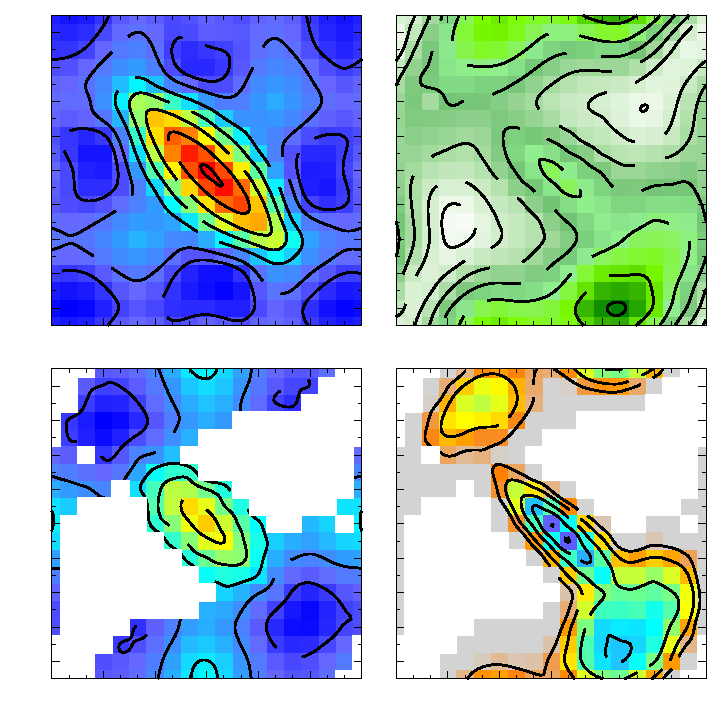
\includegraphics[width={349.00bp},height={349.00bp}]{Q1_maps}}%
    \gplfronttext
  \end{picture}%
\endgroup
